\section{Resultados.}\label{sec:4_resultados}

Los resultados aquí mostrados se engloban en dos bloques principales. Por un lado, incluimos un resumen de las condiciones óptimas de funcionamiento de la plataforma, en segundo lugar, mostramos la optimización de las concentraciones a encapsular. 

\subsection{Condiciones óptimas de funcionamiento.}\label{sec:4_resultados_puesta_a_punto}

En nuestro laboratorio disponemos de sistemas de bombas de jeringa y sistemas de control de presión de reservorios hidrostáticos. Durante las pruebas que hicimos para familiarizarnos con el funcionamiento del chip se usaron ambos sistemas y se compararon las ventajas y desventajas que ofrecían cada uno de ellos. Estas pruebas también mostraron que los flujos necesarios para formar gotas del tamaño y monodispersidad adecuados no tenían porque ser necesariamente grandes. Eran suficientes flujos de unos pocos microlitos por minuto en las dos fases para conseguir nuestro objetivo. Además, se concluyó que lo importante era la ratio entre los flujos, no tanto su magnitud.

A modo de resumen, las razones por las que se eligió el sistema de bombas de jeringa en vez del sistema de control de presión, fueron las siguientes:

\begin{itemize}

    \item Nos interesa un control del flujo, no un control de la presión. Controlar el flujo es trivial con una bomba de jeringa.
    
    \item Controlar de forma el flujo a partir ejerciendo una presión hidrostática requiere un ajuste continuo de la presión a partir de una medida continua del flujo. Debido a que la agarosa se solidifica a temperatura ambiente, no era aceptable arriesgarnos a obstruir el sensor de flujo haciendo pasar la agarosa por él, es decir, las bombas de jeringa no eran una opción para el circuito de agarosa.
    
    \item Controlar de forma manual la presión implica que en ocasiones los flujos aumenten de forma muy rápida e inesperada y perdamos la muestra en cuestión de apenas minutos.
    
    \item Las medidas con los sensores de flujo realizadas para la fase continua muestran que las bombas de jeringa son capaces de mantener flujos bajos de una forma más regular que el sistema de presión.
    
    \item Purgar los tubos resultaba una tarea engorrosa debido a las diferencias de nivel en la plataforma. Mejorar este aspecto la era uno de los objetivos cuando se diseño la platina del microscopio, sin embargo el sistema de presión esta diseñado para trabajar con tubos eppendorf en posición vertical y esto no se podía cambiar tan fácilmente. La altura de estos tubos es de 3~cm y esto provocaba el retorno del fluido al reservorio hidrostático al detener la presión.
    
\end{itemize}


Los flujos finales para hacer los encapsulados fueron 2.25~\microlitrosporminuto\ para la fase dispersa (agarosa) y 6~\microlitro\ para la fase continua (aceite). Las pruebas que se hicieron previas a los encapsulados mostraron que estos flujos se corresponden con tamaños de gotas de agarosa que rondan los 125~\micrometro. La estimación del tamaño de las gotas se hizo a partir del análisis de las imágenes de las gotas tomadas por una cámara de alta velocidad en el orificio del salida del chip. Esta estimación, sirvió para fijar el diámetro de la gota antes de empezar los experimentos de encapsulado de forma que pudimos estimar la concentración de células que debe tener la muestra a encapsular.


\subsection{Optimización de las concentraciones a encapsular.}

\subsubsection{Ajuste lineal entre los recuentos cámara de Neubauer y la densidad óptica.}

Para establecer la relación lineal entre los recuentos de células y la densidad óptica se hicieron las medidas que se muestran en la Tabla~\ref{tab:resultados_neubauer}.

\begin{spacing}{1}

\begin{table}[H]
\renewcommand\tablename{Tabla}
\renewcommand{\arraystretch}{1.5}
\centering
    
    \setlength{\extrarowheight}{-2pt}
    \begin{tabular}{ R{1.2cm} C{0.8cm} C{1.1cm} C{0.4cm} C{0.4cm} C{0.4cm} C{0.4cm} C{0.4cm} C{0.4cm} C{0.4cm} C{0.4cm} C{0.4cm} C{0.4cm} C{0.4cm} C{0.4cm} C{0.4cm} C{0.4cm} C{0.4cm} }
        \hline
        OD\small{$750$}	& Vol & D & a & b & c & d & e & f & g & h & i & j & k & l & m & n & o \\
        %\cline{1-3}
        \hline
        \hline
        

0,071	&	250	&	1	&	29	&	69	&	51	&	38	&	40	&	42	&	28	&	31	&	34	&	36	&	34	&	33	&	52	&	56	&	69	\\
0,0149	&	250	&	10	&	5	&	20	&	18	&	40	&	12	&	17	&	10	&	19	&	31	&	12	&	14	&	12	&	4	&	10	&	14	\\
0,0149	&	250	&	10	&	4	&	3	&	4	&	5	&	0	&	7	&	3	&	4	&	2	&	5	&	6	&	3	&	3	&	5	&	5	\\
0,0149	&	250	&	10	&	9	&	7	&	5	&	4	&	4	&	3	&	6	&	7	&	5	&	2	&	3	&	7	&	2	&	5	&	2	\\
0,1748	&	500	&	1	&	75	&	68	&	60	&	63	&	59	&	57	&	49	&	50	&	62	&	58	&	61	&	60	&	71	&	52	&	63	\\
0,1748	&	500	&	1	&	59	&	57	&	67	&	90	&	58	&	63	&	85	&	47	&	58	&	86	&	79	&	50	&	59	&	61	&	83	\\
0,028	&	250	&	10	&	50	&	38	&	69	&	67	&	25	&	47	&	32	&	65	&	39	&	42	&	25	&	29	&	17	&	17	&	25	\\
0,0063	&	250	&	100	&	14	&	30	&	83	&	44	&	24	&	8	&	29	&	37	&	41	&	-	&	50	&	24	&	23	&	34	&	64	\\
0,0063	&	250	&	100	&	6	&	8	&	5	&	19	&	0	&	4	&	4	&	4	&	1	&	1	&	0	&	3	&	2	&	2	&	1	\\
0,0447	&	1000	&	10	&	12	&	11	&	7	&	6	&	12	&	12	&	8	&	12	&	9	&	9	&	7	&	4	&	6	&	9	&	6	\\
0,0115	&	1000	&	100	&	2	&	3	&	2	&	3	&	3	&	5	&	4	&	1	&	6	&	4	&	3	&	7	&	3	&	1	&	3	\\
        
        \hline
    \end{tabular}

    \caption{\small Resultados de los recuentos de células realizados con la cámara de Neubauer. Cada fila contiene los datos relativos a una muestra estudiada. La primera columna empezando por la izquierda, contiene las medidas de la densidad óptica (OD) de cada una de las muestras. La segunda columna llamada  Vol, contiene el valor del volumen por el que hay que multiplicar el número de recuentos  para obtener en número de células por $\mathrm{mm^{3}}$. La tercera la dilución de la muestra y el resto de columnas contiene los valores de cada uno de los recuentos realizados.}
    \label{tab:resultados_neubauer}
    
\end{table}

\end{spacing}

Estas medidas se realizaron en el transcurso de varios días y a partir de varios cultivos diferentes.
A partir de estos datos se obtienen los valores de la Tabla~\ref{tab:analisis_neubauer}.

% \begin{table}[H]
% \renewcommand\tablename{Tabla}
% \renewcommand{\arraystretch}{1.5}
% \centering
    
%     \setlength{\extrarowheight}{-2pt}
%     \begin{tabular}{ C{2cm} C{2cm}  C{2cm} C{2cm} C{2cm} C{2cm} }
%         \hline
%         OD\small{$750$}	& $\bar{x}$ & $\sigma$ & Vol & N/cell &  $\sigma$\\
%         %\cline{1-3}
%         \hline
%         \hline
% % 0.071	&	42.8	&	250	    &	10700	&	3276	\\
% % 0.0149	&	15.9	&	250	    &	3967	&	2258	\\
% % 0.0149	&	3.9	    &	250	    &	983	    &	413	    \\
% % 0.0149	&	4.7	    &	250	    &	1183	&	520	    \\
% % 0.1748	&	60.5	&	500	    &	30267	&	3483    \\	
% % 0.1748	&	66.8	&	500	    &	33400	&	6763	\\
% % 0.028	&	39.1	&	250	    &	9783	&	4213	\\
% % 0.0063	&	36.1	&	250	    &	9017	&	4768	\\
% % 0.0063	&	4.0	    &	250	    &	1000	&	1144	\\
% % 0.0447	&	8.7	    &	1000	&	8667	&	2573	\\
% % 0.0115	&	3.3	    &	1000	&	3333	&	1619	\\



% 0.071	&	43	&	13	&	250	    &	11000	&	3000	\\
% 0.0149	&	16	&	9	&	250	    &	4000	&	2000	\\
% 0.0149	&	4	&	2	&	250	    &	1000	&	400	    \\
% 0.0149	&	5	&	2	&	250	    &	1000	&	500	    \\
% 0.1748	&	60	&	7	&	500	    &	30000	&	3000    \\	
% 0.1748	&	67	&	13	&	500	    &	33000	&	7000	\\
% 0.028	&	40	&	16	&	250	    &	10000	&	4000	\\
% 0.0063	&	36	&	19	&	250	    &	9000	&	5000	\\
% 0.0063	&	4	&	5	&	250	    &	1000	&	1000	\\
% 0.0447	&	9	&	3	&	1000	&	9000	&	3000	\\
% 0.0115	&	3	&	2	&	1000	&	3000	&	2000	\\


% 0.071	&	43	&	13	&	250	    &	11000	&	3000	\\
% 0.0149	&	16	&	9	&	250	    &	4000	&	2000	\\
% 0.0149	&	4	&	2	&	250	    &	1000	&	400	    \\
% 0.0149	&	5	&	2	&	250	    &	1000	&	500	    \\
% 0.1748	&	60	&	7	&	500	    &	30000	&	3000    \\	
% 0.1748	&	67	&	13	&	500	    &	33000	&	7000	\\
% 0.028	&	40	&	16	&	250	    &	10000	&	4000	\\
% 0.0063	&	36	&	19	&	250	    &	9000	&	5000	\\
% 0.0063	&	4	&	5	&	250	    &	1000	&	1000	\\
% 0.0447	&	9	&	3	&	1000	&	9000	&	3000	\\
% 0.0115	&	3	&	2	&	1000	&	3000	&	2000	\\

        
%         \hline
%     \end{tabular}

%     \caption{\small Datos obtenidos a partir del análisis de los datos contenidos en la Tabla~\ref{tab:resultados_neubauer}. Se vuelve a mostrar los valores de la densidad óptica y a partir de los recuentos de cada fila en la tabla anterior se calculan los valores medios, el número de células por y la desviación estándar. Los números que aparecen en la tabla se han redondeado para dejar una cifra entera en las columnas de los valores medios de los recuentos y su desviación estándar. En el caso de la densidad de células y su desviación estándar, el redondeo se ha realizado de modo que quede una cifra significativa.}
%     \label{tab:analisis_neubauer}
    
% \end{table}

\begin{spacing}{1}

\begin{table}[H]
\renewcommand\tablename{Tabla}
\renewcommand{\arraystretch}{1.5}
\centering
    
    \setlength{\extrarowheight}{-2pt}
    \begin{tabular}{ C{2cm} C{2cm}  C{2cm} C{2cm} C{2cm} C{2cm} }
        \hline
        OD\small{$750$}	& $\bar{x}$ & $\sigma$ & Vol & N$\times {10}^{3} $ &  ${\sigma}_{N} \times {10}^{3}$\\
        %\cline{1-3}
        \hline
        \hline

0.071	&	43	&	13	&	250	    &	11	&	3	\\
0.0149	&	16	&	9	&	250	    &	4	&	2	\\
0.0149	&	4	&	2	&	250	    &	1	&	0.4	    \\
0.0149	&	5	&	2	&	250	    &	1	&	0.5	    \\
0.1748	&	60	&	7	&	500	    &	30	&	3    \\	
0.1748	&	67	&	13	&	500	    &	33	&	7	\\
0.028	&	40	&	16	&	250	    &	10	&	4	\\
0.0063	&	36	&	19	&	250	    &	9	&	5	\\
0.0063	&	4	&	5	&	250	    &	1	&	1	\\
0.0447	&	9	&	3	&	1000	&	9	&	3	\\
0.0115	&	3	&	2	&	1000	&	3	&	2	\\

        \hline
    \end{tabular}

    \caption{\small Datos obtenidos a partir del análisis de los datos de la Tabla~\ref{tab:resultados_neubauer}. La columna $\bar{x}$ contiene los valores medios de los recuentos y $\sigma$ la desviación estándar de los mismos. De la misma forma N contiene los valores del número de células por $\mathrm{mm^{3}}$ contenido en las muestras y ${\sigma}_{\mathrm{N}}$ es desviación estándar de esos valores. Los valores se han redondeado para dejar una cifra entera en las columnas de los valores medios de los recuentos y su desviación estándar. En el caso de la N y su desviación estándar, el redondeo se ha realizado de modo que quede una cifra significativa.}
    \label{tab:analisis_neubauer}
    
\end{table}

\end{spacing}

A partir de la representación de los valores de la Figura~\ref{fig:recuentos_camara_neubauer}. La recta representada es un ajuste lineal a la recta $y=ax$.
%Coeficiente de determinacion
%Coefficient of determination

\begin{figure}[H]
    \begin{center}
        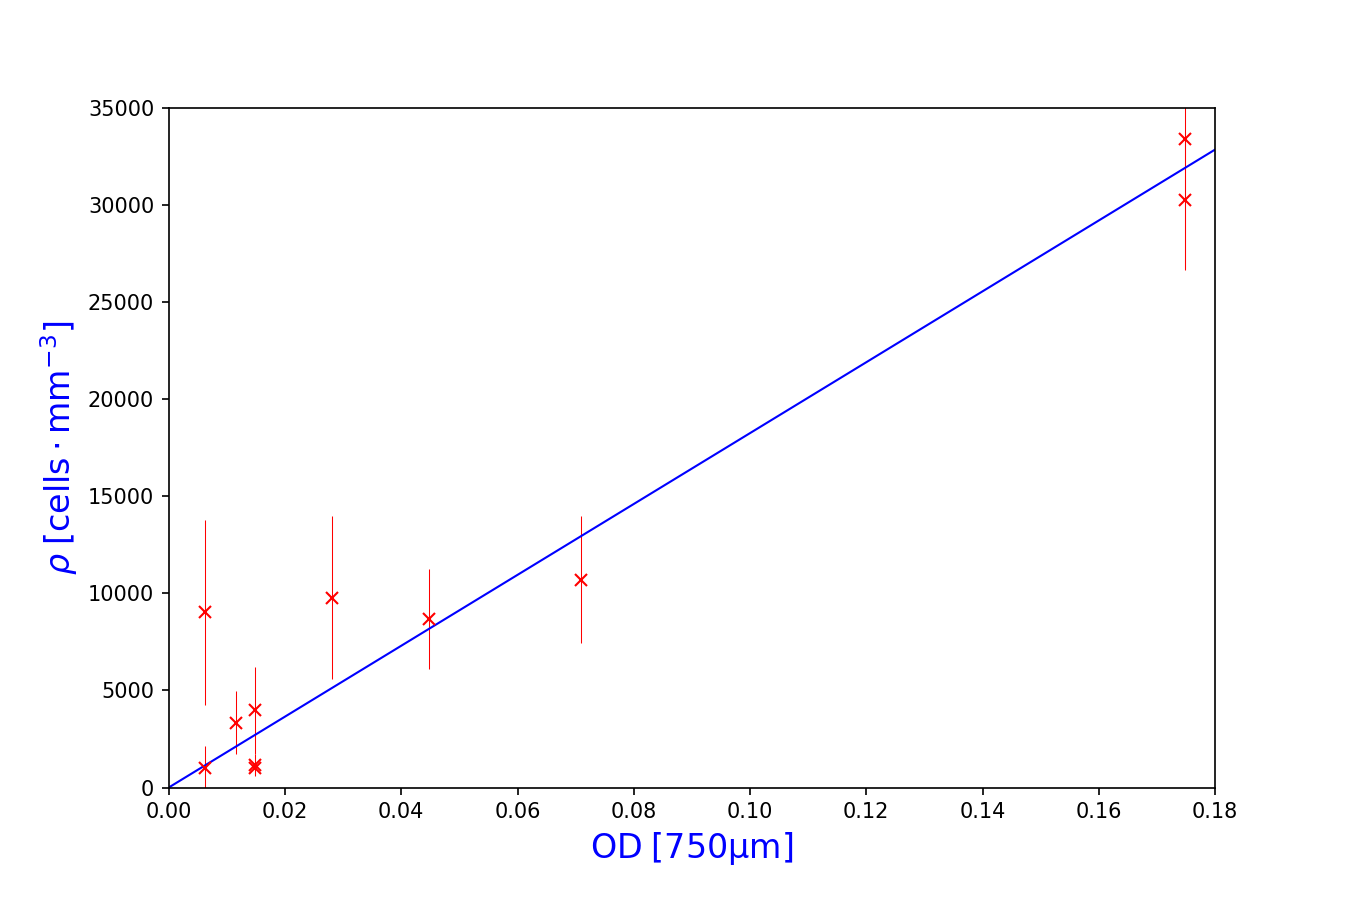
\includegraphics[width=0.8\textwidth]{4_resultados/ajuste_rho_cultivo.png}
         %\includesvg[angle=-90,height=15cm]{3_metodologia/curva_5_per_cent.svg}
        % \hspace{-17mm}{\includesvg[width=20cm]{3_metodologia/cama}}
    \caption{\small Ajuste lineal entre los recuentos cámara de Neubauer y la densidad óptica, a partir del cual se hacen las estimaciones del número de células en el cultivo. Los valores numéricos de los puntos utilizados para representar están contenidos en la Tabla~\ref{tab:analisis_neubauer}. Las barras de error se han generado a partir de los valores de la desviación estándar de los recuentos. La ecuación de la recta de ajuste es $\rho=182533\times \mathrm{OD}$. Para realizar los cálculos resulta más cómodo trabajar en ml. En ese caso la pendiente queda multiplicada por 1000.}
    \label{fig:recuentos_camara_neubauer}
    
    \end{center}
\end{figure}

El valor de la pendiente de la recta de ajuste de la figura anterior, se utilizará para calcular los valores de la concentración de células en el cultivo en la Sección~\ref{sec:resultados:encapsulados}.

\subsubsection{Encapsulados.}\label{sec:resultados:encapsulados}

Para probar que efectivamente podíamos encapsular cianobacterias con nuestro dispositivo experimental, utilizamos dos muestras con dos concentraciones diferentes. La muestra 1x tiene una concentración óptima de células para que el número de encapsulados múltiples represente el 5\% de los encapsulados totales, suponiendo un diámetro de la gota de 125~\micrometro. La muestra 10x tiene una concentración de células 10 veces superior a la muestra anterior. En ambos casos se utilizó el chip con dos entradas (ver Figura~\ref{fig:chips}) y la muestra a encapsular ya tiene células diluidas en la agarosa. Los flujos fueron $2.25~\mathrm{\mu l}$ para la fase dispersa (agarosa) y $6~\mathrm{\mu l}$ para la fase continua (aceite) que se corresponden para un diámetro de $\sim125~\mathrm{\mu m}$ como ya se ha mencionado en la Sección~\ref{sec:4_resultados_puesta_a_punto}. La temperatura a la que se mantuvo la agarosa hasta llegar al chip fue de 43~\celsius.

Ambas muestras se prepararon a partir del mismo cultivo, el mismo día. La concentración de células en la muestra original se obtuvo a partir una medida con el espectrofotómetro de 0.4832 a $750~\mathrm{\mu m}$. Teniendo en cuenta el ajuste de la Figura~\ref{fig:recuentos_camara_neubauer} se obtiene un valor de $\sim 82\cdot{10}^{6}$ cel/ml. Las dos muestras que se prepararon tenían un volumen de $\sim250~\mathrm{\mu l}$ con una concentración de agarosa de $\sim 1 \%$.

\subsubsection{Muestra 1x.}\label{muestra1x}

Supusimos, partiendo de experimentos previos que el diámetro de las gotas que se iban a formar rondaría los 125~\micrometro. Partiendo de este dato y la curva de ajuste mostrada en la Figura \ref{fig:rho_d} se estimó que la concentración de células necesaria para la distribución de encapsulados que nosotros estábamos buscando era de $\sim98\cdot{10}^{3}\;\mathrm{cel\;mm^{-3}}$ que corresponde a $1.2~\mathrm{\mu l}$ de la muestra original. Debido a que se trata de una cantidad bastante pequeña se preparó una dilución -2 a partir de la muestra original y de esta se cogieron 30~\microlitro\ que se mezclaron con 220~\microlitro\ de una dilución de agarosa al 1\%. El tiempo durante el cual se estuvieron formando \gotas\ esta entorno a los 15~min.

En la Figura~\ref{fig:imagenes_1x} se muestran dos imágenes que pretenden ser representativas de la muestra de \gotas\ obtenidas. En estas imágenes obtenidas mediante epifluorescencia, muestran una serie de puntos rojos que efectivamente se han producido los encapsulados. Lo que buscamos ahora es estudiar en que proporción se han producido los encapsulados, para saber si la muestra de gotas es la adecuada para hacer análisis genómico de las células que contienen. Para ello se va a realizar un recuento del número de gotas completas por imagen, y de estas cuantas tienen encapsulados únicos y múltiples. Los resultados obtenidos se muestran en la Tabla~\ref{tab:resultados_1x}.

\begin{figure}[H]
  \begin{center} 
  
    \subfloat[]{
     \label{subfig:1x_11}
      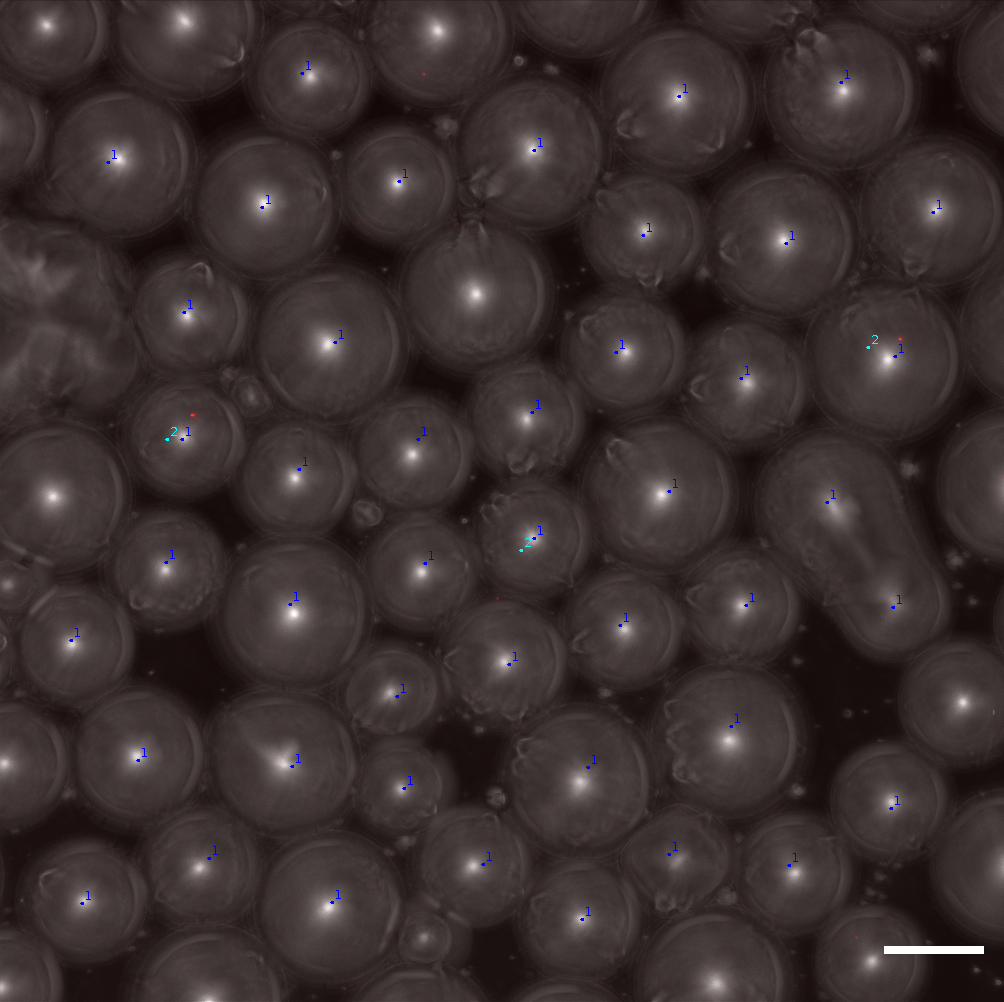
\includegraphics[width=0.4\textwidth]{4_resultados/1x_imag5_bar_scale.png}}
    \subfloat[]{
     \label{subfig:1x_12}
      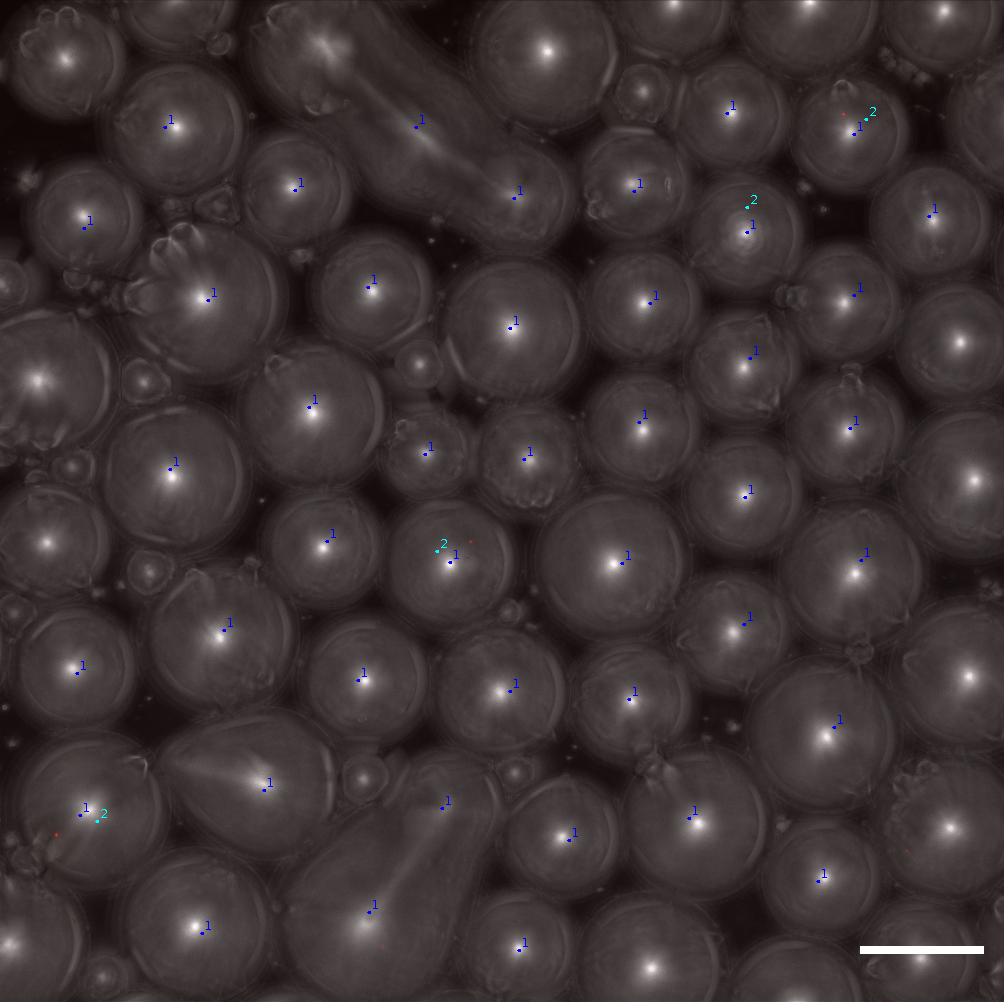
\includegraphics[width=0.4\textwidth]{4_resultados/1x_imag12_scale_bar.png}}
      
    % \subfloat[]{
    %  \label{subfig:ajuste_c}
    %   \includegraphics[width=0.5\textwidth]{4_resultados/1x_img21_recuentos.png}} 
    % \subfloat[]{
    %  \label{subfig:ajuste_d}
    %   \includegraphics[width=0.5\textwidth]{4_resultados/1x_img21_recuentos.png}} 

  \end{center}
  \vspace{-5mm}    
  \caption{\small Imágenes representativas de la muestra 1x. Las imágenes de la Figura~\ref{subfig:1x_11} y \ref{subfig:1x_12} representadas se corresponden con las imágenes llamadas 11 y 12 del a Tabla~\ref{tab:resultados_1x}. Los números que aparecen sobre las gotas hacen referencia al conteo manual que se ha realizado. El 1 indica que la gota se ha tenido en cuenta para hacer el recuento del número de gotas en la imagen. Los números mayores que 1 quieren decir que las gotas cuentan con encapsulados. El número de encapsulados es igual a número asignado menos 1. Los criterios que se han utilizado para realizar los recuentos se explican con detalle en la Sección~\ref{sec:analisis_datos}. La escala que aparece en la esquina inferior derecha representa una longitud de 100 micras en la imagen. }
  \label{fig:imagenes_1x}
\end{figure}



\begin{spacing}{1}

\begin{table}[H]
\renewcommand\tablename{Tabla}
\renewcommand{\arraystretch}{1.5}
\centering
    
    \setlength{\extrarowheight}{-2pt}
    \begin{tabular}{ C{2cm} C{2cm} C{2cm} C{2cm} C{2cm} C{2cm} }
        \hline
        Imagen	& N gotas	& 0 encap & 1 encap & 2 encap & 3 encap\\
        %\cline{1-3}
        \hline
        \hline
        
1	&	38	&	36	&	2	&	0	&	0	\\
2	&	26	&	21	&	4	&	1	&	0	\\
8	&	41	&	36	&	4	&	1	&	0	\\
9	&	46	&	40	&	6	&	0	&	0	\\
11	&	46	&	42	&	4	&	0	&	0	\\
12	&	45	&	40	&	5	&	0	&	0	\\
17	&	33	&	27	&	5	&	1	&	0	\\
18	&	9	&	8	&	1	&	0	&	0	\\
20	&	28	&	24	&	3	&	1	&	0	\\
21	&	32	&	25	&	4	&	2	&	1	\\
    
        \hline
        $\sum{x_i}$	& 344 	& 299 	& 38 	& 6 	& 1 \\
        \small{$\% \mathrm{(N\;gotas )}$}	& 100 & 87 & 11 & 2 & 0 \\
        \hline
    \end{tabular}

    \caption{\small Recuentos del número de encapsulados que se han producido en cada una de las imágenes para la muestra~1. Los valores de la columna imagen permiten identificar la imagen a partir de la cual se ha hecho cada uno de los recuentos. Por ejemplo, las imágenes 11 y 12 son las que aparecen en la Figura~\ref{subfig:1x_11} y Figura~\ref{subfig:1x_12} respectivamente. La antepenúltima fila representa el sumatorio de cada una de las columnas que se encuentran inmediatamente por encima y la última el porcentaje del sumatorio relativo a total de \gotas.}
    \label{tab:resultados_1x}
    
\end{table}
\end{spacing}

Las imágenes también nos permiten medir el tamaño de las gotas con las herramientas proporcionadas por Fiji.
Tras realizar la medida de 100 \gotas\ sobre las imágenes y suponiendo que la distribución de diámetros sigue una distribución normal tenemos que el diámetro de las \gotas\ es $102\pm16\mathrm{\mu m}$ cuando lo que esperábamos era un diámetro de la \gota\ de $\sim125\mathrm{\mu m}$.

Por tanto, llegados a este punto tenemos el recuento de los encapsulados que se han producido, una medida del tamaño de las gotas y un cálculo previo de la densidad de células de la muestra calculada a partir una medida de la densidad óptica del cultivo. También sabemos que independientemente de la concentración de células de la muestra, la proporción entre los encapsulados debe ajustarse a una distribución de Poisson y que esa distribución se caracteriza el parámetro $\lambda$. 
Lo que se hace a continuación obtener el parámetro $\lambda$ de la distribución de Poisson que mejor se ajusta a las proporciones observadas, mediante un ajuste por mínimos cuadrados. Después se obtiene la concentración de células de la muestra partiendo del parámetro $\lambda$ anterior y se compara con el $\lambda$ obtenido suponiendo la que concentración de células en la muestra era la que habíamos calculado. Los resultados de esta comparación se muestran en la Tabla~\ref{tab:comparacion_porcentajes_1x}

% Lo que se hace hace a continuación es comparar el paramentro landa de la distribución de poisson ajustada a la proporion de encapsulados observados con la distribución esperada suponiendo la concentración de celulas en la muestra y se obtiene la concentración de celulas en la muestra suponiendo un parametro landa igual al del ajuste de encapsulados observados. Los resultados de esta comparación se muestran en la Tabla~\ref{tab:comparacion_porcentajes_1x}.

\begin{spacing}{1}
\begin{table}[H]
\renewcommand\tablename{Tabla}
\renewcommand{\arraystretch}{1.5}
\centering
    
    \setlength{\extrarowheight}{-2pt}
    \begin{tabular}{C{1cm} C{1.5cm} C{2.2cm} C{1.5cm} C{1.5cm} C{1.5cm} C{1.5cm}}
        \hline
         & $\lambda$ & \small{$\rho\:(\mathrm{cel\;{mm}^{-3}})$} & 0 encap & 1 encap & 2 encap & 3 encap\\
        \hline
        \hline
        
        $r$ & 0.1286 & x & 87 & 11 & 2 & 0 \\
        $e$ & 0.0544 & 98 & 95 & 5 & 0 & 0 \\
        $a$ & 0.1291 & 233 & 88 & 11 & 1 & 0 \\
        
        \hline
    \end{tabular}

    \caption{\small Comparación los valores de $\lambda$, densidad de células en la muestra y porcentajes de los recuentos de encapsulados obtenidos a de tres formas diferentes. Las letras que aparecen en la primera columna indican si los valores de la fila pertenecen a los valores obtenidos a partir de los recuentos hechos con las imágenes $r$, los valores esperados suponiendo correcta la concentración de células de 98~$\mathrm{cel\;{mm}^{-3}}$ llamada $e$ (el Apéndice~\ref{apendice:salida} muestra las salida relativa a este cálculo) y por último los valores proporcionados por una simulación con la concentración de células de modo que el valor de $\lambda$ es el mismo al valor de la fila $a$. $\lambda$ es un valor que caracteriza a la distribución de Poisson. El valor de $\lambda$ de la fila $r$ se obtiene a partir de un ajuste por mínimos cuadrados de una distribución de Poisson multiplicada por un factor de escala a los recuentos totales del número de \gotas\ de la Tabla~\ref{tab:resultados_1x}. Todas las simulaciones parten de los valores volumen de la muestra 250~\milimetrocubico\ diámetro de la \gota\ $102\pm16$~\micrometro\ y número de simulaciones 4.}
    \label{tab:comparacion_porcentajes_1x}
    
\end{table}

\end{spacing}

Este resultado indica que la distribución de Poisson que mejor se ajusta a las proporciones observadas en la muestra es aquella con $\lambda=$0.1286 que se corresponde con una densidad de células de $\sim$233~$\mathrm{cel\;{mm}^{-3}}$ lo que supone un valor 2.4 veces superior a la concentración de células que habíamos calculado inicialmente. 

\subsubsection{Muestra 10x.}\label{muestra10x}

En el caso de la segunda muestra, el procedimiento fue el mismo que en el caso anterior. Se supuso que el tamaño de la gota seria el  mismo, 125~\micrometro, pero este caso se cogieron 30~\micrometro\ de la dilución -1 para tener una concentración de células 10 veces mayor que la muestra anterior.

De nuevo se estudian 10 imágenes y se hace un recuento del número de encapsulados que se encuentran en las \gotas\ que están completas. La Figura~\ref{fig:imagenes_10x} muestra dos de las imágenes utilizadas para hacer el recuento de las gotas y los resultados completos de este recuento se recogen en la Tabla~\ref{tab:resultados_10x}. El diámetro de las gotas en este caso es de $124\pm6$ lo cual se aproxima bastante al valor esperado. La comparación entre la distribución de Poisson que mejor se ajusta a los valores observados, los valores esperados y la concentración de células de la muestra obtenida a partir de los recuentos se recoge en la Tabla~\ref{tab:comparacion_porcentajes_10x}.

\begin{spacing}{1}
\begin{table}[H]
\renewcommand\tablename{Tabla}
\renewcommand{\arraystretch}{1.5}
\centering
    
    \setlength{\extrarowheight}{-2pt}
    \begin{tabular}{ C{1cm} C{1.5cm} C{2.2cm} C{1.5cm} C{1.5cm} C{1.5cm} C{1.5cm} C{1.5cm} C{1.5cm} }
        \hline
         & $\lambda$ & \small{$\rho\:(\mathrm{cel\;{mm}^{-3}})$} & 0 encap & 1 encap & 2 encap & 3 encap & 4 encap & 5 encap \\
        \hline
        \hline
        $r$ & 0.961 & x & 39 & 29 & 21 & 7 & 3 & 0 \\
        $e$ & 0.976 & 980 & 38 & 37 & 18 & 6 & 1 & 0 \\
        $a$ & 0.966 & 930 & 40 & 36 & 17 & 5 & 1 & 0 \\
        \hline
    \end{tabular}

    \caption{\small Comparación los valores de $\lambda$, densidad de células en la muestra y porcentajes de los recuentos de encapsulados obtenidos a de tres formas diferentes. Las letras que aparecen en la primera columna indican si los valores de la fila pertenecen a los valores obtenidos a partir de los recuentos hechos con las imágenes $r$, los valores esperados suponiendo correcta la concentración de células de 980 cel/mm3 $e$ y por ultimo los valores proporcionados por una simulación con la concentración de células de modo que el valor de $\lambda$ es el mismo al valor de la fila $a$. $\lambda$ es un valor que caracteriza a la distribución de Poisson. El valor de $\lambda$ de la fila $r$ se obtiene a partir de un ajuste por mínimos cuadrados de una distribución de Poisson multiplicada por un factor de escala a los recuentos totales del número de \gotas\ de la Tabla~\ref{tab:resultados_10x}. Todas las simulaciones parten de los valores volumen de la muestra 250~\milimetrocubico\ diámetro de la \gota\ $124\pm6$~\micrometro\ y número de simulaciones 4. }
    \label{tab:comparacion_porcentajes_10x}
    
\end{table}
\end{spacing}

En este caso la distribución de Poisson que mejor se ajusta a las proporciones observadas en la muestra es aquella con $\lambda$=0.961 que se corresponde con una densidad de células de $\sim930\;\mathrm{cel\;mm^{-3}}$ . En este caso la diferencia entre la concentración de células en la muestra que habíamos estimado previa al experimento y la calculada a partir de los encapsulados que se han producido es algo mayor a 5\%.

% \newpage

\begin{figure}[H]
  \begin{center} 
  
    \subfloat[]{
     \label{subfig:10x_a}
      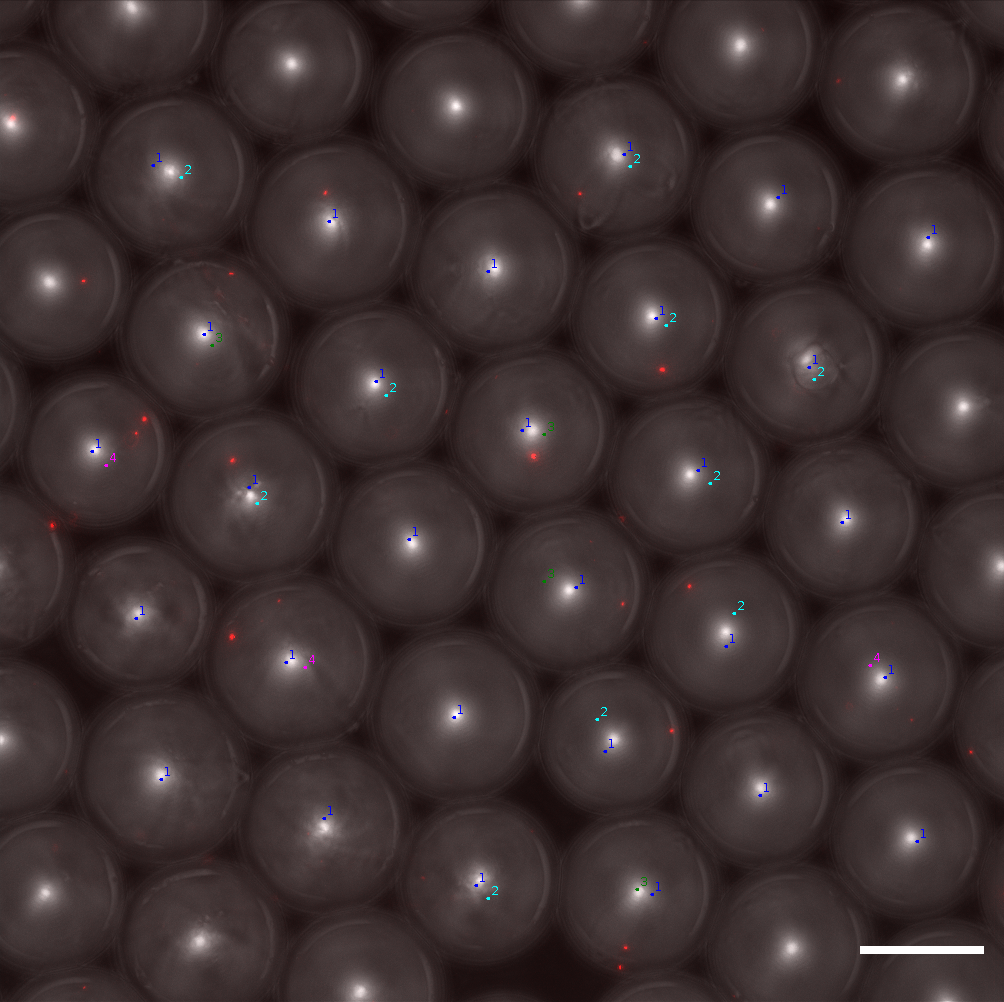
\includegraphics[width=0.45\textwidth]{4_resultados/10x_imag4_b_escala4.png}}
    \subfloat[]{
     \label{subfig:10x_b}
      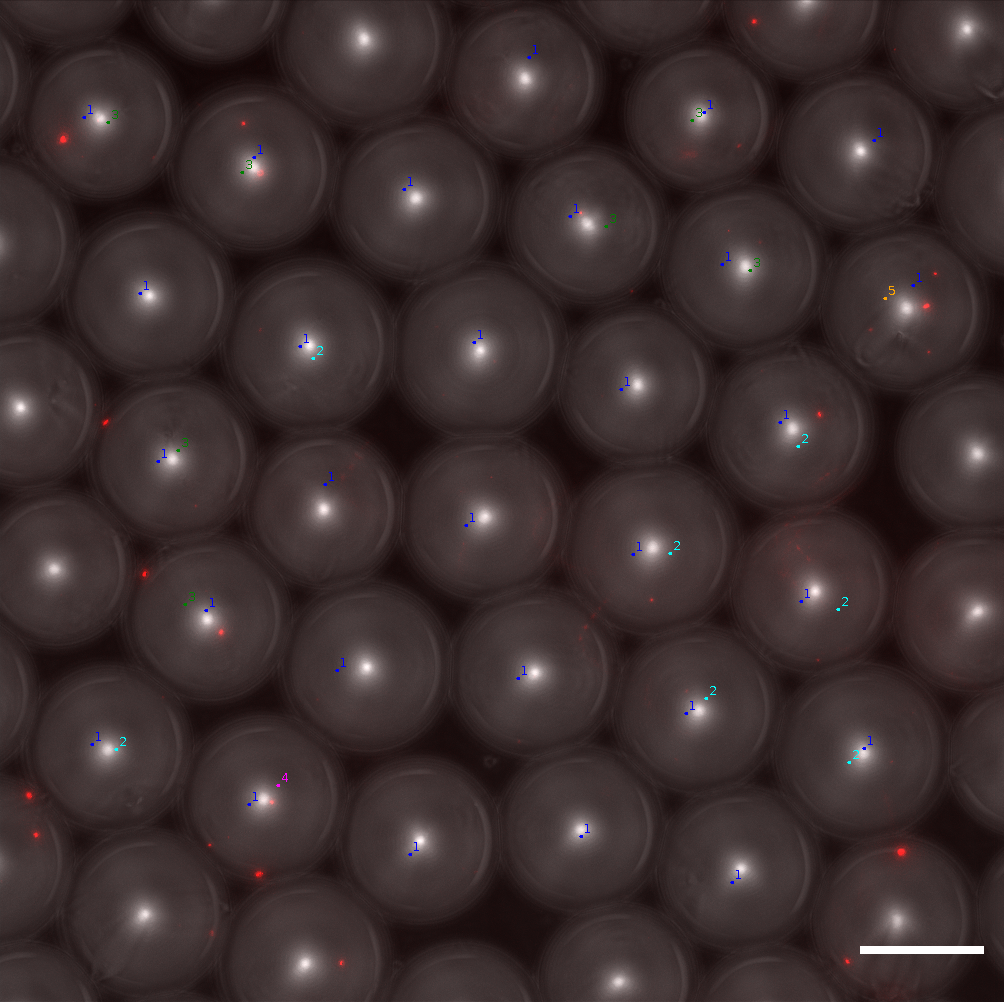
\includegraphics[width=0.45\textwidth]{4_resultados/10x_imag7_b_escala.png}}

  \end{center}
  \vspace{-5mm}    
  \caption{\small Imágenes representativas de la muestra 10x. Las imágenes de la Figura~\ref{subfig:10x_a} y \ref{subfig:10x_b} representadas se corresponden con las imágenes llamadas 2 y 7 del a Tabla~\ref{tab:resultados_10x}. De nuevo, los números que aparecen sobre las gotas hacen referencia a la conteo manual que se ha realizado. En 1 indica que la gota se ha tenido en cuenta para hacer el recuento del número de gotas en la imagen. Los números mayores que 1 quieren decir que las gotas cuentan con encapsulados. El número de encapsulados es igual a número asignado menos 1. Los criterios que se han utilizado para realizar los recuentos son los mismos que en el caso de la Figura~\ref{fig:imagenes_1x}. La escala que aparece en la esquina inferior derecha representa una longitud de 100 micras. }
  \label{fig:imagenes_10x}
\end{figure}

\begin{spacing}{1}
\begin{table}[H]
\renewcommand\tablename{Tabla}
\renewcommand{\arraystretch}{1.5}
\centering
    
    \setlength{\extrarowheight}{-2pt}
    \begin{tabular}{ C{2cm} C{2cm} C{2cm} C{2cm} C{2cm} C{2cm} C{2cm} C{2cm} }
        \hline
        Imagen	& N gotas	& 0 encap & 1 encap & 2 encap & 3 encap & 4 encap \\
        %\cline{1-3}
        \hline
        \hline
        
1	&	29	&	14	&	8	&	3	&	3	&	1	\\
2	&	28	&	14	&	8	&	4	&	2	&	0	\\
3	&	31	&	13	&	11	&	6	&	1	&	0	\\
4	&	29	&	12	&	10	&	4	&	3	&	0	\\
5	&	29	&	8	&	7	&	10	&	4	&	0	\\
6	&	27	&	7	&	11	&	5	&	1	&	3	\\
7	&	29	&	13	&	7	&	7	&	1	&	1	\\
8	&	30	&	14	&	7	&	7	&	1	&	1	\\
9	&	28	&	10	&	8	&	8	&	2	&	0	\\
10	&	28	&	8	&	7	&	8	&	3	&	2	\\

        \hline
        $\sum{x_i}$	& 288 & 113 & 84 & 62 & 21 & 8 \\
        \small{$\% \mathrm{(N\;gotas)}$}	& 100 & 39 & 29 & 21 & 7 & 3 \\
        \hline
    \end{tabular}

    \caption{\small Recuentos del número de encapsulados que se han producido en cada una de las imágenes para la muestra 10x. Los valores de la columna imagen identifican la imagen a partir de la cual se ha hecho cada uno de los recuentos. La antepenúltima fila representa el sumatorio de cada una de las columnas que se encuentran inmediatamente por encima y la última el porcentaje del sumatorio relativo a total de \gotas.}
    \label{tab:resultados_10x}
    
\end{table}
\end{spacing}

% Random seed =  7 
% $\rho$ =  980.0 1 / mm3 
% Volumen de la muestra:  250.0 mm3 
% Diámetro droplet:  124.0 micron 
% Flujo fase dispersa:  3.0 mm3 / min 
% Número de simulaciones:  4 

% Desviación estándar relativo al tamaño de la droplet expresado como tanto por 1: 0.05 

% El número de encapsulados múltiples representa el  69.936414265416 de los encapsulados únicos.

% El número de encapsulados múltiples representa el 41.154460371386605 de los encapsulados totales. Nuestro objetivo es que se encuentre en el 5\%.

% Porcentaje que representa cada conjunto de droplets con distinto número de encapsulados respecto del total de la muestra:

%  [37.67735417323904, 36.67662339218184, 17.997879536932395, 
%  5.858428141859378, 1.4495820970621005, 0.2853240794355016, 
%  0.05151407452369447, 0.006289509098823163,0.0012978352108682718, 
%  0.00019966695551819564]
 
 
 
% Lo que se parece:
 
 
 
 
%  Random seed =  7 
% ρ =  930.0 1 / mm3 
% Vol_muestra:  250.0 mm3 
% Diametro droplet:  124.0 micron 
% Flujo fase dispersa:  3.0 mm3 / min 
% Número de simulaciones:  4 
% Desviación estandar relativo al tamaño de la droplet expresado como tanto por 1: 0.05 

% El número de encapsulados multiples representa el  65.0325772431116 % de los encapsulados únicos.

% El número de encapsulados multiples representa el 39.40590296139609 % de los encapsulados totales. Nuestro objetivo es que se encuentre en el 5%.

% Porcentaje que representa cada conjunto de droplets con distinto número de encapsulados respecto del total de la muestra:
%  [39.59241778075934, 36.60403389397352, 17.014371396169757, 5.276566518120976, 1.24586707556663, 0.21942434552046897, 0.040929927963326784, 0.006988036481543597, 0.00039931637037391983, 9.982909259347996e-05]